%\documentclass[
%	12pt,
%	a4paper,
%	bibtotoc,
%	cleardoubleempty, 
%	idxtotoc,
%	ngerman,
%	openright
%	final,
%	listof=nochaptergap,
%	]{scrbook}
\renewcommand{\baselinestretch}{1.5} 
%\usepackage[T1]{fontenc}
%\usepackage[utf8]{inputenc}
%\usepackage[pdftex]{graphicx}
%\usepackage{float}
%\begin{document}

\chapter{Algorithmus}
\section{Was macht der Algorithmus?}
Der Algorithmus läuft auf dem Raspberry Pi in einem eigenen Thread. Seine Aufgabe ist es, die Route des Zuges anhand der Eingabe zu berechnen, eine Folge von Anweisungen für den Zug zu erstellen und diese eine nach der anderen dem Zug über Socket-Kanal mithilfe vom Speaker Thread mitzuteilen. Eine weitere Aufgabe des Algorithmus ist es, die aktuelle Position des Zuges nach jeder Änderung während der Fahrt zu ermitteln und danach zu überprüfen, ob es Abweichungen von der geplannten Strecke gibt. Solche Anweisungen muss der Algorithmus berücksichtigen und entsprechend handeln, in dem er die Strecke anpasst, falls notwendig, und eine neue Folge von Anweisungen erstellt.\\
\section{Definitionen der Schlüsselwörter}
\label{chap:alg_keywords}
\textit{\textbf{Bahnhof, Zwischenhaltestelle, Position des Zuges}}: Sowohl ein Bahnhof, als auch eine Zwischenhaltestelle entsprechen einem (aus 8 im Projekt vorhandenen) RFID-Tag, den der Zug erkennen kann und wessen "Name" (und somit seine Position) der Zug dem Pi mitteilt. Ein Bahnhof wird von einer Zwischenhaltestelle dadurch unterschieden, dass auf einem Bahnhof ein sinnvolles Anhalten stattfinden kann: Damit der Zug Reisende aufnimmt bzw. ihnen die Möglichkeit gibt, auszusteigen. Aus Bequemlichkeit sind die Bahnhöfe im Bereich [0, 3] mit natürlichen Zahlen durchnummeriert (dadurch kann man die entsprechende Zeile bzw. Spalte in der Matrix ansprechen), während die Zwischenhaltestellen 0.5, 1.5 usw. heißen. Die Zwischenhaltestellen sind lediglich für die Anweisungen, die der Pi erstellt, notwendig: Der Zug wird seine Geschwindigkeit bei einer Zwischenhaltestelle runtersetzen, falls er bei dem folgenden Bahnhof anhalten muss. Außerdem könnte man diese Zwischenhaltestelle für eine niedrigere Geschwindigkeit bei gefährlichen Kurwen verwenden: Bei manchen Zwischenhaltestellen festlegen, dass der Zug dort immer langsam fahren muss.\\
\\
Dabei ist es zu beachten, dass die Zahlen 0.5, 1.5 usw. vom Typ double sind. Zwei double Werte soll man aufgrund der Rundungsfehler und der eingeschränkten Genauigkeit nie vergleichen: Die Gleitkommazahlen, die auf dem Papier gleich sind, werden auf verschiedenen Geräten unterschiedlich dargestellt. So könnte eine Zahl 0.125 auf dem Gerät-1 binär anders aussehen, als dieselbe Zahl auf dem Gerät-2. Das Problem läßt sich allerdings durch Mapping lösen (man kann zum Beispiel mit integer Werten arbeiten und 0, 5, 10, 15, usw. anstatt 0, 0.5, 1, 1.5, usw. verwenden). In dieser Dokumentation werden die Stationen deshalb aus Bequemlichkeit weiter als 0, 0.5, 1, 1.5 usw. bezeichnet. Dies erleichtet auch die Arithmetik bei der Hauptaufgabe des Algorithmus, nämlich bei der Erstellung der Anweisungen. Weitere Information darüber findet man in der Beschreibung der \textit{createOrderlist()} - Methode.\\
\begin{figure}[H]	
\caption{Route (Fahrt im Uhrzeigersinn)}
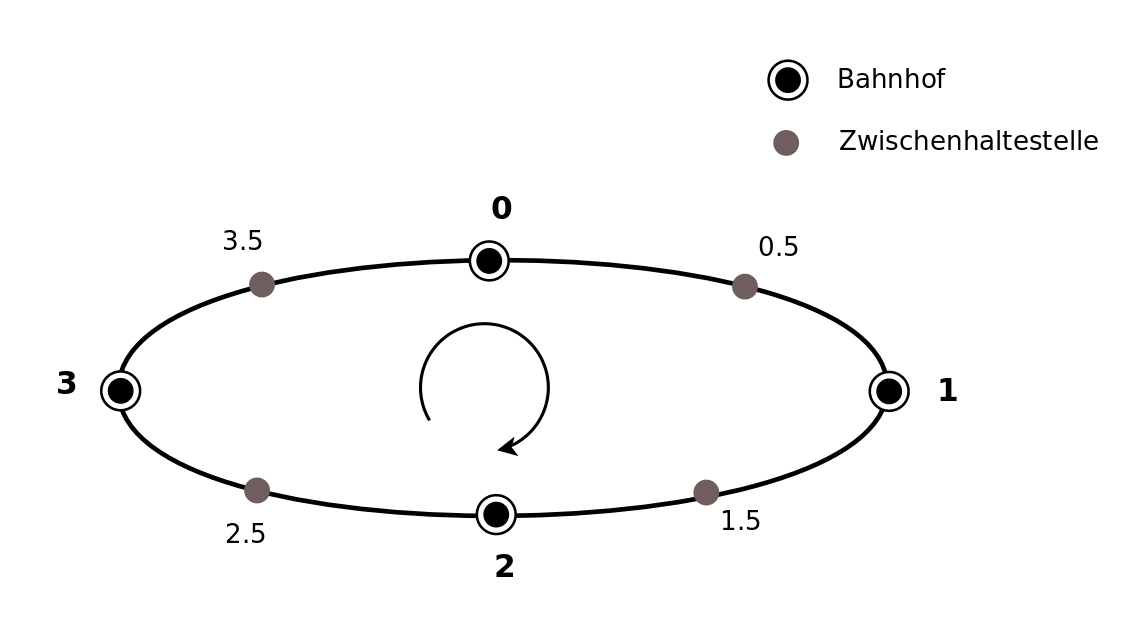
\includegraphics[width=2\textwidth, width=470pt]{content/images/route.png}
\label{pic:route}
\end{figure}
\noindent
\textit{\textbf{Start-Bahnhof}}: Dies ist der Bahnhof, an dem der Zug nach dem Start des System ankommt. Diese Position wird auch als erste dem Algorithmus auf der Pi-Seite mitgeteilt.\\
\\
\textit{\textbf{Anweisung}}: Eine Anweisung besteht aus drei Teilen: einer Vor-Geschwindigkeit (weiter hier VG, im Code das Attribut \textit{beforeSpeed}), einem Tag, und einer Nach-Geschwindigkeit (weiter hier NG, im Code das Attribut \textit{afterSpeed}). Die VG wird auf der Zug-Seite sofort nach dem Eingang der Anweisung als die aktuelle Geschwindigkeit des Zuges gesetzt. Sowohl der Tag, als auch die NG werden auf der Zug-Seite temporär gespeichert. Nachdem der Zug eine Zeit gefahren ist und ein neuer Tag erkannt wurde, wird der Wert des ermittelten Tags mit dem gespeicherten Tag verglichen. So erkennt man eine Abweichung im Verhalten des Zuges. Falls keine Abweichung gibt und der erwartete Tag ermittelt wurde, wird die NG als aktuelle Geschwindigkeit gesetzt und die Position (der Tag) des Zuges wird dem Pi mitgeteilt.\\ 
\\
\textit{Beispiel-Anweisungen:} (2,0.5,1): "Fahre mit Geschwindigkeit 2 bis zum Tag 0.5, danach setze die Geschwindigkeit auf 1". Der erste Wert - 2 - wird danach (auf der Zug-Seite) auf eine schnelle Geschwindigkeit abgebildet, der letzte - 1 - auf eine langsame Geschwindigkeit.\\
(1,1,0): "Fahre mit Geschwindigkeit 1 bis zum Tag 1, danach setze die Geschwindigkeit auf 0". Bei Geschwindigkeit gleich 0 hält der Zug an.\\
\begin{figure}[H]	
\caption{Anweisung}
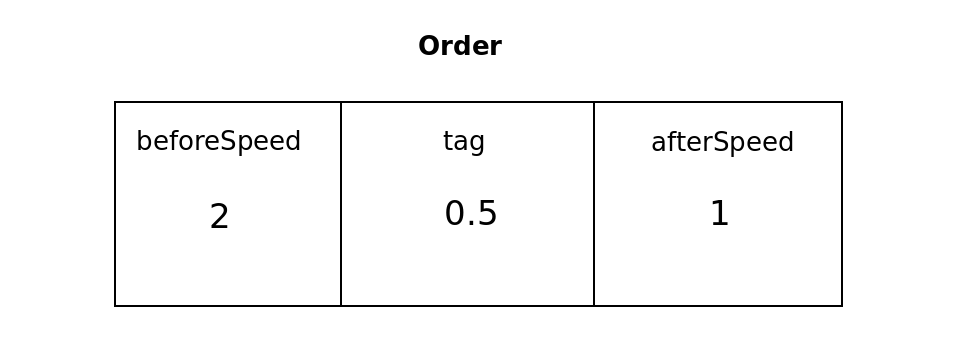
\includegraphics[width=2\textwidth, width=330pt]{content/images/order.png}
\label{pic:anweisung}
\end{figure}
\noindent
%
\section{Detaillierte Beschreibung/Ablauf}
Der Grund dafür, dass der Algorithmus in einem eigenen Thread läuft, besteht darin, dass Raspberry Pi gleichzeitig in der Lage sein muss, mit dem Zug zu kommunizieren. Dies geschieht über Socket-Kommunikation, für welche Listener und Speaker Threads auf der Pi-Seite verantwortlich sind, die ensprechend die Informationen vom Zug erhalten (nämlich die Position des Zuges, das macht Listener Thread vom Pi) und Daten dem Zug mitteilen (nämlich die neue Anweisung, das macht Speaker Thread vom Pi). \\
%
\begin{figure}[H]	
\caption{Kommunikation zwischen dem Zug und dem Raspberry Pi}
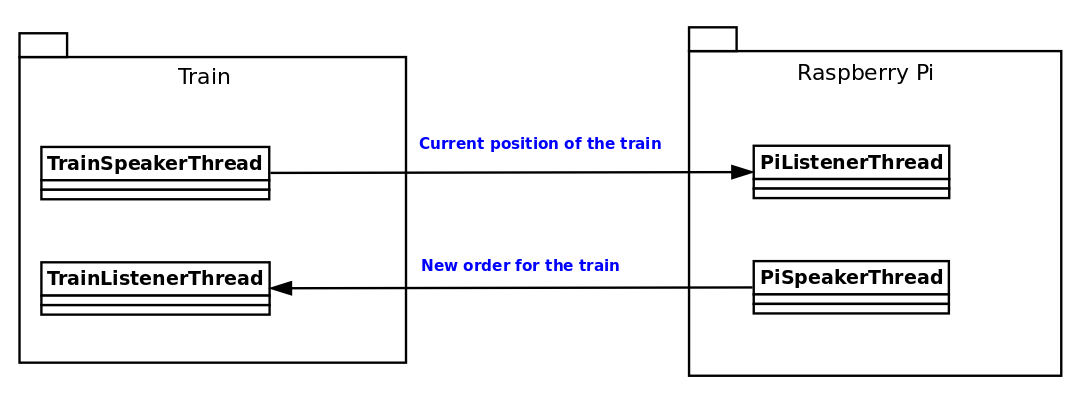
\includegraphics[width=2\textwidth, width=470pt]{content/images/communication.png}
\label{pic:communication}
\end{figure}
\noindent
Die Eingabe, die der Algorithmus bearbeiten muss, beinhaltet die Information über die Anzahl der Reisenden, ihren Abfahrtbahnhof und ihren Zielbahnhof. Dies kann für Bequemlichkeit in der Form einer Matrix gespeichert werden:\\
\\
\\
\begin{table}[H]
\caption{Szenario 1}
\center
 \begin{tabular}{|c|c|c|c|c|}
 \hline
  Von/Nach & B0 & B1 & B2 & B3 \\ \hline
  B0 & 0 & 0 & 3 & 0\\   \hline
    B1 & 0 & 0 & 0 & 7 \\   \hline
      B2 & 0 & 0 & 0 & 0\\   \hline
        B3 & 0 & 0 & 2 & 0 \\   \hline
 \end{tabular}
\end{table}
\noindent
\\
Die oben angegebene Tabelle ist folgend zu verstehen:\\
\\
- 3 Reisende wollen vom Bahnhof0 zum Bahnhof2 fahren\\
- 7 Reisende wollen vom Bahnhof1 zum Bahnhof3 fahren\\
- 2 Reisende wollen vom Bahnhof3 zum Bahnhof2 fahren\\

\begin{figure}[H]	
\caption{Szenario 1}
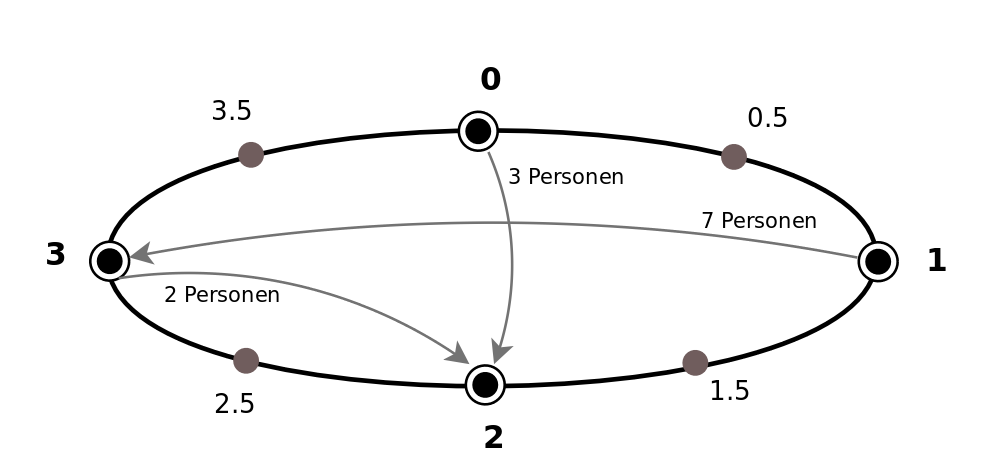
\includegraphics[width=2\textwidth, width=470pt]{content/images/szenario1.png}
\label{pic:szenario1}
\end{figure}


\section{Zusammenhang von den Methoden des Threads PiAlgorithm}
%Ablauf seiner Arbeit
Bevor man Anweisungen für den Zug erstellt, ist es sinnvoll zu wissen, wo der Zug sich befindet (die ursprüngliche Position beim Anschalten). Im oben beschriebenen Szenario 1, z.B., ist es einfach zu bemerken, dass der Zug sich unterschiedlich verhalten soll, wenn er beim Bahnhof 0 oder Bahnhof 1 startet. So muss er im ersten Fall (Start beim Bahnhof 0) während der Fahrt in seinem ersten Kreis beim Bahnhof 2 anhalten, damit die Reisende, die er am Bahnhof 0 aufgenommen hat, aussteigen können. Im zweiten Fall (Start beim Bahnhof 1) gibt es keinen Grund für das Anhalten am Bahnhof 2, da der Zug weder Reisende hat, die dort aussteigen möchten, noch gibt es an dem Bahnhof Reisende, die einsteigen möchten.\\
Deshalb fährt der Zug nach dem Anschalten bis zu dem ersten Bahnhof (keine Zwischenhaltestelle) und hält dort an. Semantische Bedeutung dieser Aktion mit dem Übertrag auf die Realität kann man als die Möglichkeit für die Mitarbeiter, einzusteigen, sehen. Der Raspberry Pi wartet so lange: Der Algorithmus führt lediglich eine Anweisung in seiner Methode \textit{readTrainPosition()} aus und wird blockiert, so lange die Position noch nicht ermittelt wurde (dies ist ausführlich im Kapitel \textit{Semaphore} beschrieben). Nachdem die Position in \textit{TrainPos} dank dem PiListenerThread gespeichert wurde, wacht der Algorithmus auf und berechnet die Route mithilfe von \textit{createOrderlist()}-Methode. Er erstellt eine Reihe von Anweisungen, die den Zug an richtigen Stationen anhalten und später weiter bewegen, damit alle Reisende an ihr Ziel kommen. Dieser Verlauf wird unten in einem Aktivitätsdiagramm dargestellt, während die Methoden durch eine textuelle Beschreibung repräsentiert werden.\\
\begin{figure}[H]	
\caption{Erste Fahrt}
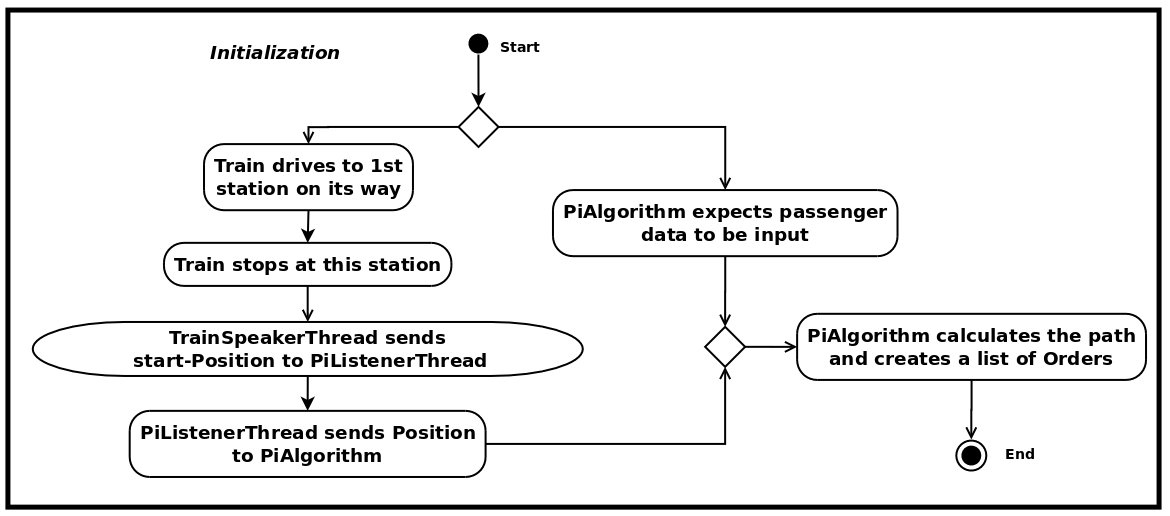
\includegraphics[width=2\textwidth, width=470pt]{content/images/Act-dia1.png}
\label{pic:init}
\end{figure}
%
\noindent
Im guten Szenario (so lange alle RFID-Tags vom Zug richtig erkannt werden) muss der Algorithmus die Liste von Anweisungen lediglich einmal erstellen; ansonsten wird die Methode \textit{repairOrderlist()} aufgerufen, die die createOrderlist()-Methode wieder verwendet und die neue Reihe von Anweisungen erstellt. Der Pi sendet mithilfe von PiSpeakerThread immer nur eine Anweisung und wartet, bis die geschickte Position (Tag) vom Zug erreicht und dem PiListenerThread mitgeteilt wird. Wenn sie übereinstimmen, ist alles in Ordnung und die nächste Anweisung kann geschickt werden, bis die Liste von Anweisungen leer wird.\\
\\
Das unten angegebene Diagramm stellt den Zusammenhang zwischen den Methoden und deren Reihenfolge grafisch dar. \\
\begin{figure}[H]	
\caption{Der gewöhnliche Verlauf}
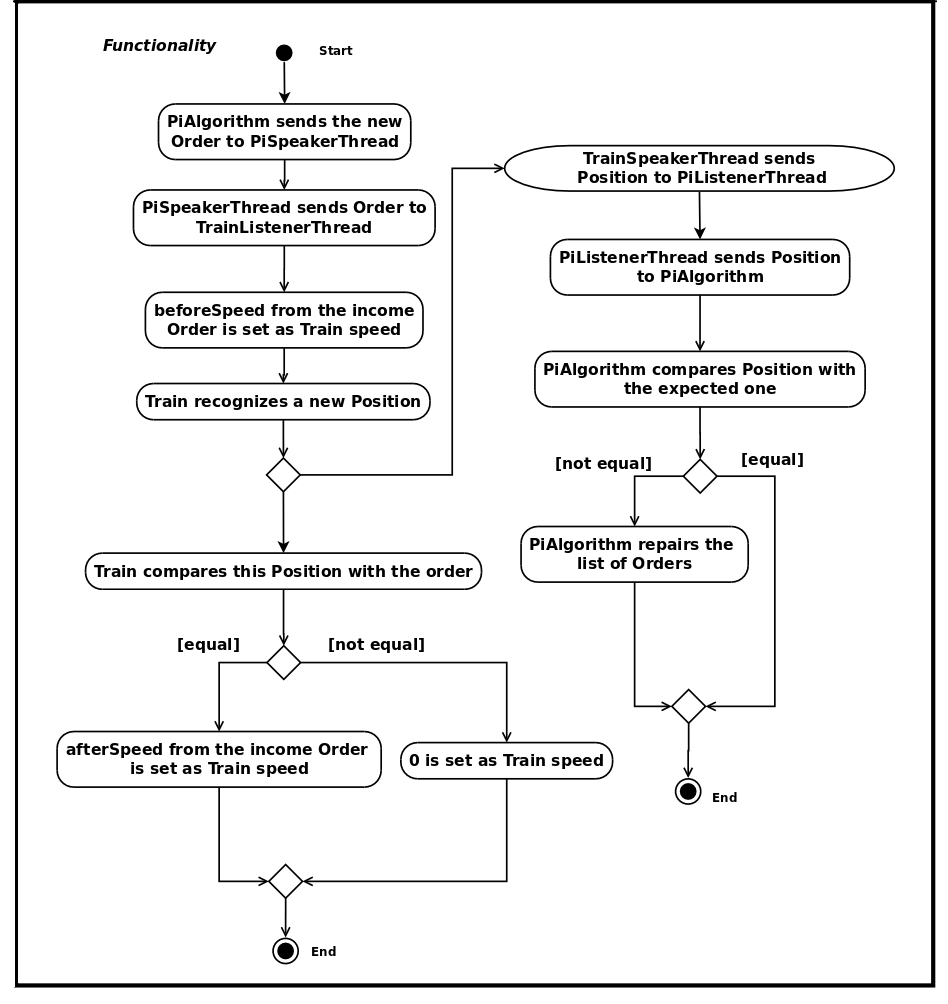
\includegraphics[width=2\textwidth, width=470pt]{content/images/Act-dia2.png}
\label{pic:init}
\end{figure}
%
\begin{figure}[H]	
\caption{Klassendiagramm}
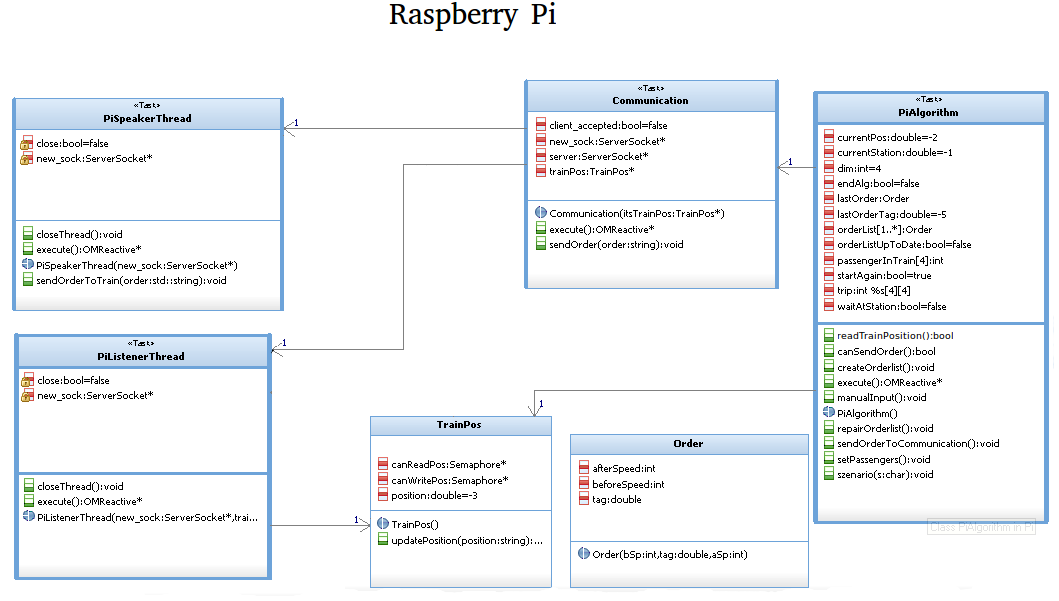
\includegraphics[width=2\textwidth, width=470pt]{content/images/RaspberryPi.png}
\label{pic:init}
\end{figure}
%
\section{createOrderList() - Methode}
Der Algorithmus wurde von uns komplett entwickelt. Die Hauptaufgabe des Algorithmus ist die Berechnung der Liste von Anweisungen. Sobald diese vorhanden ist, bleibt es lediglich, die Anweisungen aus der Liste eine nach der anderen dem Zug zu schicken, bis die Liste leer ist. Wenn die Liste leer geworden ist und die letzte Anweisung dem Zug geschickt wurde, hat der Raspberry Pi seine Arbeit gemacht. Er teilt das dem Nutzer mit und ist bereit, neue Aufgaben zu bekommen (neue Eingaben der Reisende aufzunehmen). Die Start-Position ist dem Zug bereits bekannt - dies ist die letzte Position, die der Zug dem Pi beim Erreichen der Endstation mitteilt. So kann man auf die Fahrt zum ersten Bahnhof, die der Zug immer nach dem Start des Systems gemacht hat, verzichten.\\
\\
Dabei sind folgende Bemerkungen wichtig:\\
\\
1) Die Matrix wird als ein zweidimensionaler Array implementiert.\\
\\
2) Die Einträge, die sich auf der Hauptdiagonale der Matrix befinden, sollen gleich 0 sein und ignoriert werden. In der Realität macht es keinen Sinn, Reisende zu haben, die vom Bahnhof 0 zum Bahnhof 0, d.h. einen vollen Kreis, fahren. In der \textit{createOrderlist()}-Methode werden solche Einträge deshalb ignoriert. Bei der Eingabe des Nutzers wird eine Meldung ausgegeben, falls ein Eintrag auf der Hauptdiagonale ungleich 0 ist, und ein solcher Eintrag wird auf 0 gesetzt - lediglich für die genaue Darstellung, denn diese Einträge werden gar nicht berücksichtigt.\\
\\
3) Die längste Strecke, die der Zug fahren kann, ist beim Start am Bahnhof 0 gleich einem vollen Kreis und danach bis zum Bahnhof 2 (genau 1.5 Kreise). Dies lässt sich folgend erklären: Alle Reisende, die Bahnhöfe 3 und 0 erreichen müssen, können das bereits beim ersten Kreis machen. Es bleiben Reisende, die vom Bahnhof 2 zum Bahnhof 1, und die vom Bahnhof 3 zu den Bahnhöfen 1 und 2 fahren müssen. Im allgemeinen (wichtig für die mögliche Vergrößerung der Anzahl von Stationen) fährt der Zug am längsten \textit{(einen vollen Kreis) + bis zu dem (N-2)-ten Bahnhof nach dem Start-Bahnhof,} wo N die Anzahl der Bahnhöfen darstellt. In unserem Fall (4 Bahnhöfe) entspricht das \textit{einem Kreis + bis zu dem (4-2)-ten (=2.ten) Bahnhof.}\\
\\
4) Die Anweisungen für die Zwischenhaltenstellen sind von den Anweisungen für die Bahnhöfe abhängig und lassen sich aus diesen erstellen. Beispiel aus dem Szenario 1: Der Zug startet am Bahnhof 0 und hält weiter an Bahnhöfen 1, 2 und 3. Danach fährt er allerdings am Bahnhof 0 durch. Dies bedeutet, der Zug kann an der Zwischenhaltestelle 3.5 schneller fahren.\\
\\
5) Der Algorithmus arbeitet mit der Dimension der Matrix \textit{dim=N} und ist somit flexibel - er kann auf eine Matrix beliebiger Größe eingesetzt werden.\\
\\
6) Die Hauptdiagonale der Matrix ist "flexibel" - dies ist für die Logik der \textit{createOrderlist()}-Methode wichtig. Aus Bequemlichkeit betrachten wir das Beispiel mit dem Start am Bahnhof 0. So sieht die Diagonale gewöhnlich aus. Bei einem Start, z.B., am Bahnhof 2, wird sie allerdings "versetzt" und somit folgendermaßen aussehen:\\
\\
\begin{figure}[H]	
\caption{Versetzung der Hauptdiagonale}
\center
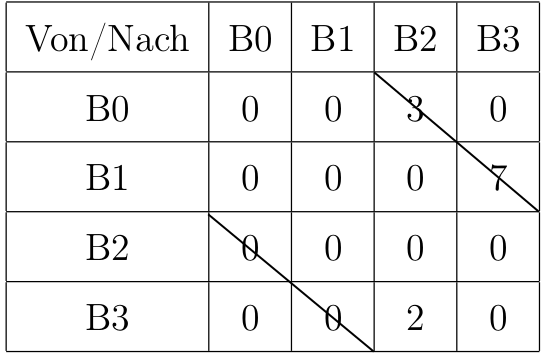
\includegraphics[width=2\textwidth, width=270pt]{content/images/matrix2.png}
\label{pic:DiagonaleVersetzt}
\end{figure}
\noindent
Damit man die Versetzung der Hauptdiagonale besser versteht, kann man sich die vorgenommene Transformation der Matrix folgend vorstellen: Die ersten zwei Zeilen werden ausgeschnitten und nach der Zeile "B2" hinzugefügt. So definiert die Startposition des Zuges immer die "pseudo-erste" Zeile der Matrix. Dabei werden die Elemente in der Matrix nicht unnötig kopiert - die Iteration durch die Matrix wird später lediglich anhand des Modulo-Operators angepasst. Aus Bequemlichkeit betrachten wir nun das Beispiel, in dem der Zug am Bahnhof 0 startet.\\
\\
\textit{\textbf{Wie erstellt der Algorithmus die Liste von Anweisungen?}\\}
\\
Dies lässt sich anhand der Matrix für das oben beschriebene Szenario 1 erklären.\\
\begin{figure}[H]	
\caption{Matrix mit einer Hauptdiagonale}
\center
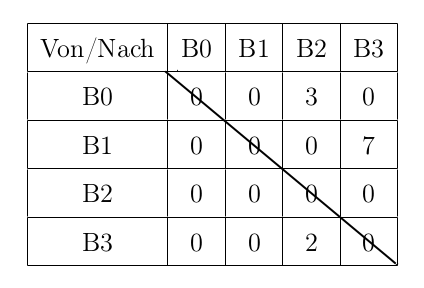
\includegraphics[width=2\textwidth, width=310pt]{content/images/matrix.png}
\label{pic:Hauptdiagonale}
\end{figure}
\noindent
Es wird ein Hilfsfeld \textit{stop} erstellt. Seine Länge ist (2*N - 2); es enthält boolesche Elemente, die mit "false" initialisiert werden. "False" entspricht dabei der Anweisung "do not stop", d.h. der Zug fährt an dem RFID-Tag weiter. Das erste Element (mit Index 0) im Feld \textit{stop} entspricht dabei dem Bahnhof, der gleich nach dem Start-Bahnhof kommt (in unserem Fall also dem Bahnhof 1), das zweite (Index 1) - dem weiteren Bahnhof (Bahnhof 2), usw. Das N-te Element (Index N-1) entspricht dem Start-Bahnhof, allerdings nach einem vollen Kreis. Deshalb muss man die beiden Hälften des Feldes unterschiedlich bearbeiten.\\
\\
Die Matrix wird dreimal durchgelaufen.\\
1) Beim 1. Durchlauf wird lediglich die "pseudo-erste" (in diesem Fall tatsächlich die erste) Zeile analysiert, nämlich die Zeile "B0". Alle Einträge, die ungleich 0 sind, verlangen vom Zug das Anhalten noch im ersten Kreis (genauer gesprochen, ist diese Strecke genau 1 Station kleiner, als ein voller Kreis) am Bahnhof, der dem Index der Spalte entspricht. In unserem Fall ist das Spalte "B2". Deshalb wird stop[1] gleich "true".\\
\\
2) Beim 2. Durchlauf (getrennt vom 1. Durchlauf nur für die Lesbarkeit, hat dasselbe Zweck und kann zusammengefasst werden) werden alle Einträge über der (pseudo-) Hauptdiagonale berücksichtigt. Die Zeile, die mindestens einen nicht leeren Eintrag hat, setzt das Element mit dem entsprechenden Index in \textit{stop} auf "true". In unserem Fall ist das die Zeile B1. Deshalb wird stop[0] gleich "true". Es wird auch stop[2] (entspricht Bahnhof 3) auf "true" gesetzt, da dies der Zielbahnhof der Reisende vom Bahnhof 1 ist. Die Spalte hat also den gleichen Einfluss.\\
\\
3) Beim 3. Durchlauf werden die Elemente unter der Hauptdiagonale berücksichtigt. Während die Durchläufe 1) und 2) immer für die Strecke \textit{(Vollkreis - 1 Station)} verantwortlich sind, erledigt der 3. Durchlauf die letzte Hälfte des Feldes \textit{stop}. So wird der Eintrag "2" in der Zeile "B3" dazu führen, dass das Element stop[2] (nochmal!) auf "true" gesetzt wird (allgemein notwendig, obwohl man am Bahnhof 3 schon anhält - ein Zufall dank dem Eintrag in der Zeile "B1", das wird nicht immer so sein). Außerdem wird stop[5] auf "true" gesetzt: Bahnhof "B2" muss erreicht werden.\\
\\
4) Nun muss man das letzte Element mit dem Wert "true" in \textit{stop} finden. Dies ist die Endstation des Zuges. Falls ein solches gar nicht vorhanden ist, hat der Zug laut der Eingabe des Nutzers nichts zu tun. In unserem Fall sieht das Feld \textit{stop} folgendermaßen aus:\\
\begin{figure}[H]	
\caption{Hilfsfeld \textit{stop}}
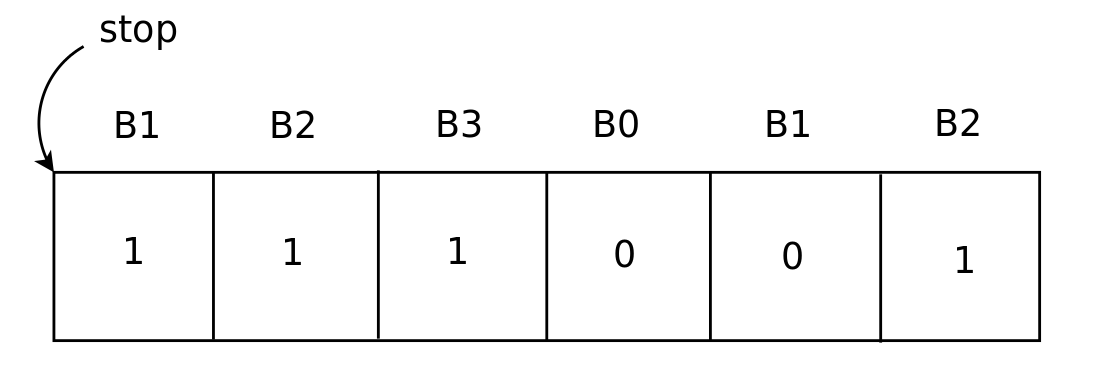
\includegraphics[width=2\textwidth, width=290pt]{content/images/stop1.png}
\label{pic:stop1}
\end{figure}
\noindent
5) Anhand der Einträge im Feld \textit{stop} kann man nun die Anweisungen erstellen. Nämlich werden für jedes Element (bis zu der Endstation) aus \textit{stop} zwei Anweisungen erstellt: Für die Zwischenhaltestelle und für den Bahnhof. Die Geschwindigkeiten sind folgend definiert: "low" (gleich 1), falls der Zug nach dem Anhalten vom Bahnhof erst startet oder nach der Zwischenhaltestelle an einem Bahnhof anhalten muss; "0", falls der Zug an dem RFID-Tag anhalten soll (dies macht nur bei \textit{afterSpeed} Sinn); ansonsten "high" (gleich 2), was einer hohen Geschwindigkeit entspricht. Die tatsächliche Geschwindigkeit wird auf der Zug-Seite definiert. So abstrahiert der Algorithmus von den technischen Details des Zuges und arbeitet nur mit für ihn verständlichen Geschwindigkeiten "schnell", "langsam", und "stehen bleiben".\\
\\
Eine grafische Darstellung der Liste mit Anweisungen \textit{orderList} findet man unten für das Hilfsfeld \textit{stop} für das zweite Szenario.\\
%to edit
\\
Im \textit{zweiten Szenario} möchten lediglich drei Reisende vom Bahnhof 0 zum Bahnhof 2 fahren.\\
\begin{table}[H]
\caption{Szenario 2}
\center
 \begin{tabular}{|c|c|c|c|c|}
 \hline
  Von/Nach & B0 & B1 & B2 & B3 \\ \hline
  B0 & 0 & 0 & 3 & 0\\   \hline
    B1 & 0 & 0 & 0 & 0 \\   \hline
      B2 & 0 & 0 & 0 & 0\\   \hline
        B3 & 0 & 0 & 0 & 0 \\   \hline
 \end{tabular}
\end{table}
\noindent
Damit die Aufgabe schwieriger wird und gleichzeitig um den oben genannten Ansatz zu erklären, werden wir als Start-Position den Bahnhof 1 betrachten.\\
\\
\begin{figure}[H]	
\caption{Szenario 2}
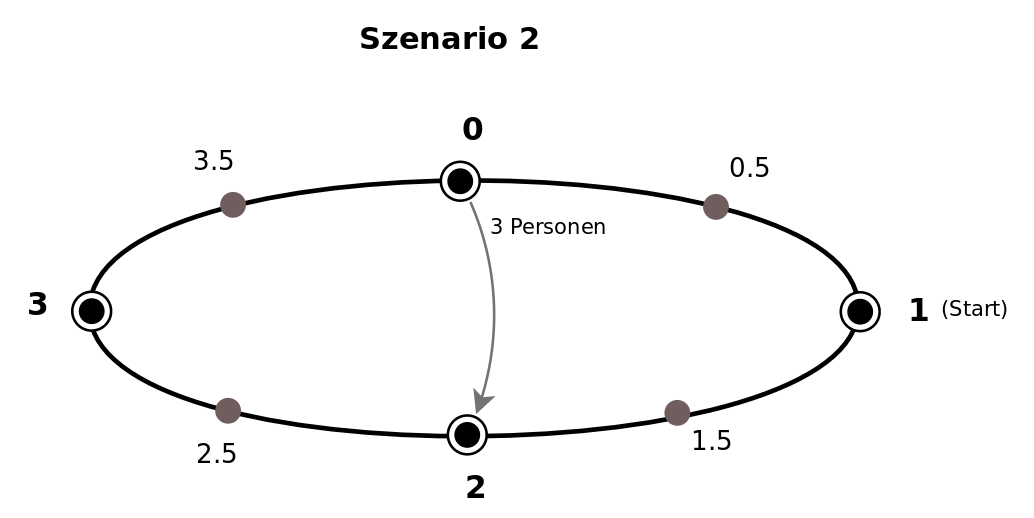
\includegraphics[width=2\textwidth, width=450pt]{content/images/szenario2.png}
\label{pic:szenario2}
\end{figure}
\noindent
Die Liste der Anweisungen \textit{orderList} und das Feld \textit{stop} sehen in diesem Fall folgendermaßen aus:\\
\begin{figure}[H]	
\caption{\textit{orderList} für Szenario 2}
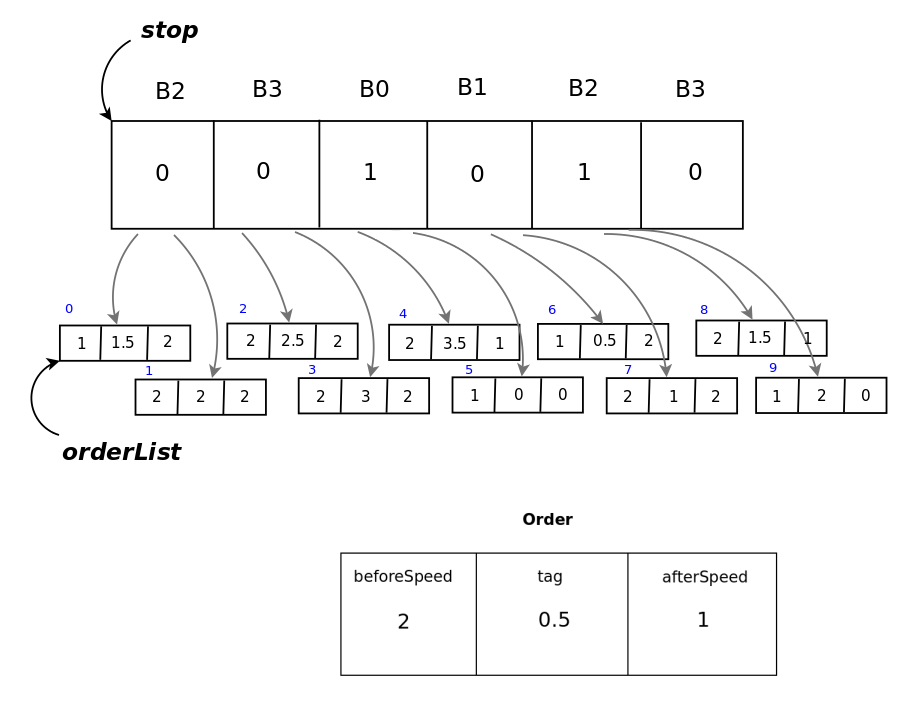
\includegraphics[width=2\textwidth, width=430pt]{content/images/orderList.png}
\label{pic:orderList2}
\end{figure}
\noindent
Man sieht aus den Anweisungen, dass der Zug langsam startet: Mit Geschwindigkeit "1" bis zum Tag "1.5". Dort setzt er sie auf "2" und fährt so bis zum Tag "3.5". Ab dort muss er langsamer fahren: Er kommt einem Bahnhof nah, bei dem er anhalten soll - Bahnhof 0. Dort steigen Reisende ein und der Zug fährt langsam ab. Beim Tag "0.5" darf er wieder schneller werden und fährt deshalb mit "2" bis zum Tag "1.5", wo er wieder langsamer (\textit{afterSpeed} gleich "1") wird. Am Tag "2" bleibt der Zug stehen - dies ist seine Endstation.\\
\section{Laufzeit und alternative Ansätze für die Implementierung}
%Laufzeit
Die \textbf{\textit{Laufzeit des Algorithmus}} ist folgendermaßen definiert:\\
$T = O( (n-1) + (n-1)*(n/2) + (n-1)*(n/2) ) = O(n^2)$\\
\\
Dabei wurde von den Entwicklern überlegt und diskutiert, ob der Algorithmus am Anfang die Route komplett berechnen und erst dann die erste Anweisung dem Zug schicken soll oder jedes Mal, wenn die Position des Zuges ihm mitgeteilt wurde überprüfen soll, was der Zug als nächstes zu tun hat. Es wurde die erste Variante gewählt und implementiert, welche als Vorteil die Eigenschaft hat, dass der Algorithmus ohne Verzögerung, die für die Berechnung notwendig ist, die nächste Anweisung dem Zug mitteilen kann. Als Kritik kann man den Punkt nennen, dass die Verzögerung am Anfang sich sammelt und dadurch größer ist. Außerdem soll die zweite Variante genommen werden, falls man häufige Änderungen (neue Eingaben der Reisende) erwartet. Diese Überlegungen sind allerdings nur für sehr große Dimensionen der Matrix wichtig und haben somit für die Geschwindigkeit in diesem Projekt keine Relevanz.\\
\\
Darüber hinaus wurde diskutiert, ob man zusätzlich zu der Matrix bzw. an ihrer Stelle eine verkettete Liste verweden könnte. Dies scheint den Algorithmus in dem Fall, dass der Zug auch im inneren Kreis fahren können soll, zu vereinfachen. So sind in diesem Fall an bestimmten Stellen Verzweigungen der Strecke möglich. Allerdings ist die Matrix lediglich eine Art der Darstellung von den Eingaben des Nutzers und lässt sich weiter beliebig anpassen und bearbeiten. So könnte man zwei weitere Zeilen B4 und B5 hinzufügen und vereinbaren, dass es vom Bahnhof 0 sowohl zum Bahnhof 1 (Zeile B1), als auch zum Bahnhof 5 (Zeile B5) einen Weg gibt.\\
%
%
\section{repairOrderList() - Methode}
Es kann passieren, dass der Zug einen RFID-Tag überfährt, ohne ihn zu erkennen. Der Zug wird in diesem Fall einen "falschen" Tag lesen und dem Algorithmus diesen Tag mitteilen, während er selbst nicht weiter fährt (ein Sicherheitsmechanismus). Der Algorithmus muss diese Abweichung behandeln. Dafür wird im Zug ein Buch über die Reisende geführt, die sich gerade im Zug befinden, zusammen mit ihren gewünschten Zielbahnhöfen. Wenn Reisende in den Zug einsteigen, werden sie aus der Matrix gelöscht. Wenn die Reisende aus dem Zug aussteigen, werden sie auch aus dem Buch im Zug gelöscht. So kann man bei einer Abweichung immer erkennen, wer noch an Stationen wartet und wer sich im Zug befindet (und wo er oder sie hin möchte). Eine neue Ausführung der Methode \textit{createOrderlist()} "repariert" die Liste mit Anweisungen. Dies ist nicht immer notwendig: Vielleicht hat der Zug eine Zwischenhaltestelle nicht erkannt und dort nicht langsamer bzw. schneller geworden?. Oder der Zug ist an Stationen vorbei gefahren, wo er nicht anhalten musste? In diesem Fall muss man eine neue Liste nicht erstellen, sondern man muss nur eine bzw. einige Anweisungen (die schon jedenfalls zufällig vom Zug durch Vorbeifahren ausgeführt wurden) aus der Liste entfernen, ohne diese dem Zug zu schicken. Die \textit{repairOrderlist()}-Methode kann somit verbessert werden. Bei unserer Anzahl der Bahnhöfe ist das unwichtig; bei einer großen Matrix lässt sich die Rechenzeit somit sparen.\\
%
%
%
%\begin{figure}[H]	
%\caption{...}
%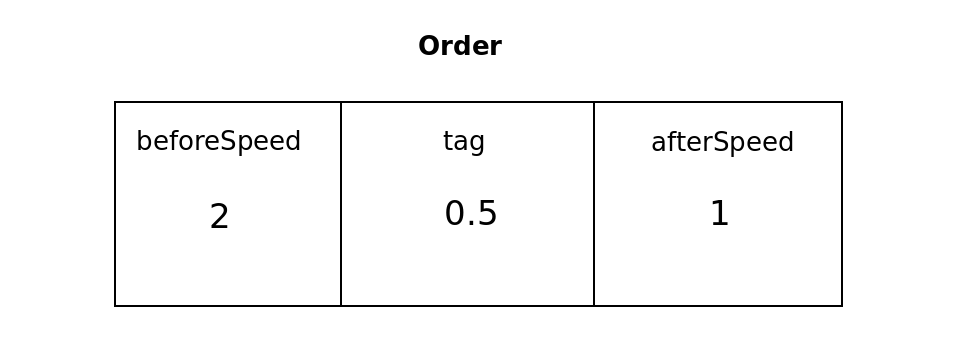
\includegraphics[width=2\textwidth, width=470pt]{content/images/order.png}
%\label{pic:pi_communication}
%\end{figure}
%
\chapter{Semaphore}
Die Semaphore und ihr Einsatz werden anhand der Implementierung an der Pi-Seite erklärt.\\
\\
Nachdem der Algorithmus die Eingaben des Nutzers gespeichert hat, braucht er die Start-Position des Zuges, damit er die Liste von Anweisungen erstellen kann. Diese erfährt er mithilfe von der Methode \textit{readTrainPosition()}. Der Wert darf allerdings erst dann gelesen werden, wenn der Zug ihn dem PiListenerThread mitgeteilt hat. Bevor das passiert, darf der Algorithmus nichts machen und muss blockiert sein. Die einfache Lösung, die sich anbieten könnte, besteht darin, dass man eine weitere Methode \textit{algorithmCanRead()} hinzufügt, die ein "Flag" - eine boolesche Variable überprüft, die vom PiListenerThread auf "erlaubt" gesetzt wird, sobald die Position aktualisiert wurde. Der Algorithmus liest die Position und setzt das "Flag" selbst auf "nicht erlaubt" - damit er sie nicht wieder liest, bevor eine neue Position vom Zug mitgeteilt worden ist. Das Wort "blockiert" ist hier entscheidend. Wie oft soll das "Flag" überprüft werden? Wie lange soll der Algorithmus blockiert werden? Wie bekommt er rechtzeitig mit, dass die Position aktualisiert wurde? Der oben genannte Ansatz verlängt Polling, d.h. Ressourcen(Rechenzeit)-Verschwendung. Die richtige Lösung an dieser Stelle ist der Einsatz von Semaphoren.\\
\\
Rhapsody bietet eine Factory von Semaphoren an. Ein Factory-Objekt verfügt über eine Methode \textit{createOMOSSemaphore()}, die den Zeiger auf eine neuerstellte Semaphore zurückliefert. Bei der Erzeugung kann man definieren, ob die Semaphore frei ist oder blockieren soll (das Attribut \textit{initialCount}, by default gleich 1) und wie groß der maximale Wert (das Attribut \textit{maxCount}, bezeichnet die Anzahl von Ressourcen, by default auch 1) sein soll. Die Semaphore bietet die Methoden \textit{p()} (Ressource nehmen) und \textit{v()} (Ressource freigeben), die hier \textit{wait(-1)} und \textit{signal()} genannt werden. Wenn ein Thread \textit{wait(-1)} aufruft, während \textit{initialCount} den Wert 0 hat (keine Ressourcen vorhanden), wird er blockiert. \textit{Signal}() blockiert, wenn \textit{initialCount} gleich \textit{maxCount} ist, allerdings nicht bei allen Plattformen.\\
In unserem Fall ist es wichtig, dass signal() auch blockiert, denn wir wollen nicht, dass der PiListenerThread die Position des Zuges aktualisiert, bevor der Algorithmus (der aus irgendwelchem Grund zu langsam war) die alte Position einmal gelesen hat. Dies würde dazu führen, dass der Algorithmus nicht mitbekommt, dass der Zug da war, wo er sein musste, und dass der Zug seine Position richtig erkannt hat, und es wird \textit{repairOrderlist}()-Methode aufgerufen.\\
\\
Wir wollen von OMOSSemaphoren abstrahieren und erstellen deshalb eine eigene Klasse Semaphore, die Methoden \textit{request()} (die bekannte Methode p() ) und \textit{release()} (die Methode r() ) enthält. Wir brauchen zwei Objekte (bzw. Zeiger) dieser Klasse, die in der Klasse \textit{TrainPos} als Attribute vorhanden sind: \textit{canReadPos} und \textit{canWritePos}.\\
\\
\textit{canReadPos} ist am Anfang blockiert, falls der Algorithmus \textit{request}() aufruft: Man darf noch nicht lesen. Der Zug teilt seine Position mit und der PiListenerThread aktualisiert sie (\textit{canWritePos} erlaubt ihm, \textit{request}() aufzurufen), zusätzlich ruft er \textit{release}() für \textit{canReadPos}. Nun wäre PiListenerThread blockiert, falls er gleich wieder \textit{request}() für \textit{canWritePos} aufruft. Er muss warten, bis der Algorithmus die Position einmal gelesen und \textit{release}() für \textit{canWritePos} aufgerufen hat.\\
\\
Aus dieser Beschreibung des gewünschten Verlaufs ist es klar, dass wir die Semaphore \textit{canReadPos} und \textit{canWritePos} folgend initialisieren müssen: (initialCount=0, maxCount=1) für den ersten und (initialCount=1, maxCount=1) für den zweiten.\\
%\end{document}